%!TEX root = thesis.tex
%% %% ***************** Research materials and methods *****************

%% ************************************************ 3 ************************************************

\section{Research material and methods}\label{sec:research-material-and-methods}

In the next section
we explain in more detail
what the data used in the study
consists of
and what methods were used
in attempt to answer the research goals.
The content of the section is briefly described below,
and the steps of the research are explained.

The data in the research is mainly made of two parts.
The most important part is, obviously,
the log data produced by the numerous RPA processes.
The second data part,
complementing the study,
is the support ticket data written by clerks of customer banks.
In order to use the data safely in the cloud environment
it was necessary to sanitize the data
from any sensitive information.
This was done by anonymizing the log data
and using only timestamps from the support tickets.

After confirming the results of anonymization,
the data was preprocessed into a better format
to make it more usable by algorithms.
More processing was done inside the pipeline
as ML Studio offered several usable components for this
but main cleaning was easier to execute in local environment.
This was also done with PowerShell scripting.

The actual ML pipeline structure
is discussed in the next section.

%% ************************************************************************************************************

\subsection{Support ticket data}\label{subsec:meth-efecte-ticket-data}

Like all other software,
RPA components fail from time to time.
As described before,
RPA logs are verbose
making possible error identification from among them hard.
Due to that,
it is not feasible to create log parsers
that would be able to identify critical errors
from within thousands of lines of log.
When critical error happens
causing the RPA process to fail,
the banking clerks need to finish manually
the job left by the RPA robot.
Every time this happens,
these clerks then send a support request ticket
to Samlink technical help desk
and ask to fix the issue.

When clerks send the ticket to technical support,
a verbose description of the situation is written
to help developers to identify the problem.
This description often contains sensitive end customer information
like bank account details and social security numbers.
To avoid privacy issues when processing this data,
it was decided to use only timestamps of the tickets.
The resulting data was practically a list of date and time values.
More about the issue from privacy point of view
is described in section~\ref{subsec:meth-data-anonymization}.

%% ************************************************************************************************************

\subsection{RPA log data}\label{subsec:meth-rpa-log-data}
Robotic process algorithms used in Samlink
are designed to ease the workload of bank clerks.
RPA robots work in behalf of bank clerks
executing routine tasks that require mostly manual labor.

Like other software,
RPA also produces log data during runtime.
As dozens of RPA automations are running
in several bank environments
the amount of log entries produced is also significant,
up to over a million lines per week.
This log data is not in consistent structure
as it is formed out of typical CSV data
and injected with even more inconsistent JSON data
that varies in contents vastly.
Example of log data after anonymization phase
can be seen in the appendix~\ref{sec:app-log-data-input}.

RPA log data is stored in SQL database.
The database is split in live production log
that is gathered for two weeks
and then moved to archive
that has several years worth of log.
In this study we used archived data
as it was easier to acquire in one run
without the need to merge different parts together.
Archive also had amount of data
that was considered sufficient
for machine learning algorithm training,
with data entries spanning almost two and a half years
and rowcount exceeding 80 million.

Samlink RPA logs have few standard fields.
These are listed in a table~\ref{tab:log-row-fields}.
The most notable aspects here
are the fields named message and rawmessage.

\textit{Message} holds the short log message
written by the RPA agent during automation execution.
This includes details about the issue,
what part of the process failed,
and possible stack trace of the error.

\textit{Rawmessage} is JSON-formatted representation
of all the default features,
including the message
and multiple other additional features
that RPA agent is able to output regarding the log event.
These additional fields are what vary from log entry to log entry.
Some of the possible fields are shown in a table~\ref{tab:log-row-fields},
but several other field types exist.
JSON data in them can be nested in multiple layers,
as seen in the appendix~\ref{sec:app-log-data-input}.

\begin{table}[]
    \centering
    \begin{tabular}{|L{0.25\textwidth}|L{0.25\textwidth}|L{0.5\textwidth}|}
        \hline
        \textbf{Field}    & \textbf{Contents}                               & \textbf{Examples}                                                             \\ \hline
        organizationUnitId & Samlink organization unit                       & 5                                                                            \\ \hline
        level              & Log level                                       & Information | Warning | Error | etc.                                         \\ \hline
        logType            & Type of log entry                               & Default | User                                                               \\ \hline
        timeStamp          & Date and time for log entry                     & 2019-09-10T03:00:01.6278373+03:00                                            \\ \hline
        fingerprint        & Unique identifier for log entry                 & bcd51984-agdc-40a6-b571-y6a97f98a4e3                                         \\ \hline
        machineName        & Workstation name of the RPA agent               & T2490A1011                                                                   \\ \hline
        processName        & Name of the RPA automation                      & RPA-bank-hakemusten-tietojen-siirto\_Samlink Production                      \\ \hline
        jobId              & Identifier for current RPA automation execution & 24a84531-010b-457f-90t1-5ayc98d7b557                                         \\ \hline
        robotName          & Name of the agent executing automation          & RPA-BANK-1-1234                                                              \\ \hline
        machineId          & Workstation ID number                           & 5                                                                            \\ \hline
        message            & Short message regarding the entry               & Throw exception: Saldo ei riitä | \newline Tarkistettiin A:n nimi                    \\ \hline
        rawmessage         & JSON formatted message including most of the columns above and several more fields regarding the log entry &
        \{
        \textbf{"message"}: "Siirryttiin Varallisuus-sivulle.",\newline
        \textbf{"level"}: "Information",\newline
        \textbf{"logType"}: "User",\newline
        \textbf{"timeStamp"}: "2019-09-10T03:00:50.6103121+03:00",\newline
        \textbf{"fingerprint"}: "70f44345-22bb-46df-885e-75f180fc4d48",\newline
        \textbf{"windowsIdentity"}: "LOCAL\textbackslash{}\textbackslash{}T123456",\newline
        \textbf{"machineName"}: "T2490A1011",\newline
        \textbf{"processName"}: "RPA-bank-hakemusten-tietojen-siirto\_Samlink Production",\newline
        \textbf{"processVersion"}: "1.0.7111.31245",\newline
        \textbf{"jobId"}: "24a84531-010b-457f-90t1-5ayc98d7b557",\newline
        \textbf{"robotName"}: "RPA-BANK-1-1234",\newline
        \textbf{"machineId"}: 11,\newline
        \textbf{"fileName"}: "LisaaTiedot\_Talous\_Varat",\newline
        \textbf{"logF\_BusinessProcessName"}: "rpa-sp-011-OTT-valmistelu"  \}
        \\ \hline
    \end{tabular}
    \caption{Log fields in RPA log data}
    \label{tab:log-row-fields}
\end{table}

Without rawmessage,
the data was in pure CSV-format
and could have been more easily processable from the start.
However,
it was not certain
that rawmessage would not hold usable data for ML
as in some cases plain message-field did not include
all the most interesting keywords that were present
in the extra fields of rawmessage.
Nevertheless,
using rawmessage in anomaly detection
posed another problem.

When feeding the log data to anomaly detection algorithm,
it was crucial that all the rows were as minimally unique as possible
in order to use the pattern finding abilities of the algorithm.
Too unique data points would have made all of them anomalies
compared to each other.
Because rawmessage included other column data in a long text format,
certain unique information such as fingerprint and timestamp
were necessary to remove from within the data manually,
as they could not be extracted easily
with tools in Azure ML Studio
during ML pipeline execution.
Thus,
it was seen easier to preprocess the data
with another script in local environment
before exporting it to the cloud.
The final script is presented in the appendix~\ref{sec:app-data-cleaning-script}.
When training ML algorithm with rawmessage,
timestamp and job ID values were included retrospectively
from their corresponding columns outside rawmessage.


%% ************************************************************************************************************

\subsection{Data anonymization}\label{subsec:meth-data-anonymization}

\subsubsection*{Support ticket data privacy}
Samlink handles highly sensitive banking customer data in its processes,
such as personal identification numbers, home addresses, email addresses and bank account numbers.
All possibly sensitive data had to be removed
before data could be transferred out from production environment to cloud.
Due to bureaucratic reasons,
technical support tickets were under more strict policies.
Because of this,
they were allowed to be used in the research
on condition that no business critical nor customer sensitive information
was processed in the first place.
Only way to assure this
was to select solely timestamp fields from ticket data.
Thus, no sanitation for ticket data was needed
as ticket data consisted of only list of datetime values.

%% ............................................................................................................

\subsubsection*{RPA log data sanitization}
Information privacy is one of the key values in Samlink business promise
as company develops high security banking applications
and processes sensitive customer data.
Thus, several aspects were needed to take into consideration
before log data could be authorized for thesis study usage.
To improve privacy,
it was decided to assume
that personal customer details are not critical information
for ML algorithm training
if goal is to find possible problems in RPA runtime
and not detect individual customer related problems.
Also,
as mentioned in section~\ref{subsec:bg-data-sensitivity},
all customer and user related information was excluded from support ticket data,
making individual customer information redundant in the log data.
Thus,
it was not necessary to achieve just adequate security
by less safe and more effort consuming ways
such as pseudonymization or k-anonymization
(explained in the section~\ref{subsec:bg-data-sensitivity}),
which would have also required strict inspections
before data could have been approved for cloud processing.

During thesis kickoff,
several sensitive information types were recognized from the log data,
and all possible types and their different forms were considered
before anonymization script was approved to be used in production environment.
Anonymization was executed by replacing sensitive information
with general pattern describing the replaced information type.
With this,
it was at least possible to keep the information
whether a log row had included customer sensitive data,
and what type of data was involved.
Thus,
it was theoretically still possible to recognize repeating anomalies
that had, for example,
social security number included in the log event.
List of considered sensitive info types, their examples,
as well as values replacing the sensitive data
has been listed in the table~\ref{tab:regex-sensitive-info}.

\begin{table}[]\small
    \tabcolsep=0.11cm
    \begin{tabularx}{\textwidth}{|L{0.17\textwidth}|L{0.27\textwidth}|L{0.30\textwidth}|Y|}
        \hline
        \textbf{Info type} &
        \textbf{Example} &
        \textbf{Replaced value} &
        \textbf{Comment}
        \\ \hline
        Social security number &
        010190-0123 &
        10105051470101 &
        Includes '-','+' and 'a' format
        \\ \hline
        Email &
        author@thesis.fi &
        EmailAddress0101 &
        \\ \hline
        IBAN number &
        FI8612345600000123 &
        1010IBANnumber0101 &
        Only Finnish format
        \\ \hline
        BBAN number with dash &
        123456-123 &
        1010BBANnumber0101 &
        \\ \hline
        Phonenumber, international &
        +358501234567 &
        1010PhoneNumberInt0101 &
        With or without whitespaces
        \\ \hline
        Phonenumber, local &
        050-1234567 &
        1010980230101 &
        With or without whitespaces or dashes
        \\ \hline
        Business ID &
        1234567-8 &
        1010BusinessID0101 &
        Finnish format
        \\ \hline
        Business ID, international &
        FI12345678 &
        101086512350101 &
        \\ \hline
        Business ID, int.\ zero form &
        0012345678 &
        1010865123500101 &
        \\ \hline
        Credit card number &
        4920191061682346 &
        1010664900101 &
        \\ \hline
        Windows Identity &
        K123456 &
        1010WinID0101 &
        Used in company processes
        \\ \hline
        Address, common &
        Teekkarikuja 1 a 42 &
        1010AddressCommon0101 &
        Common street name endings
        \\ \hline
        Address, ZIP &
        Bulevardi 2 B 69, 00100 &
        1010AddressZip0101 &
        Disregards city name after ZIP
        \\ \hline
        Bank ID &
        12345678 &
        10108426100101 &
        Bank user ID
        \\ \hline
        BBAN without dash &
        12345600000123 &
        101088420101 &
        \\ \hline
        Artificial business ID &
        8123456789 &
        101086512354970101 &
        Used in RPA processes
        \\ \hline
    \end{tabularx}
    \caption{Information replaced with Regex search from log data.
        Data values are replaced with patterns with numbers or numbers and letters
        depending on the original format in the data.
        Patterns are formatted uniquely so that they can be recognized amongst the anonymized data,
        each starting with 1010 and ending with 0101,
        and having a typewise identifier in the middle.
        With numeric patters,
        numbers are selected as letter representations,
        like business ID = 8651235 (BUSINES)}
    \label{tab:regex-sensitive-info}
\end{table}

Script searched for repeating patterns related to sensitive information types.
This was done with regular expression, or regex, searching.
With regular expressions,
different repeating patterns can be extracted and replaced from the data.
Each sensitive data type has some sort of unifying feature,
such as string length, number of digits, or location of certain character.\cite{li2008regular}
Some types are clear and standardised like social security number
(6 numbers, '-', '+' or 'a', three numbers and a number or a letter),
or credit card number (15-16 numbers),
while with some other types it may be hard
to take all possibilities into consideration,
like address (one or more words, at least one number,
possibly one letter or more in case of 'apartment' or 'apt', more numbers \etc).
Still,
most of the cases could be considered to a degree
that was deemed satisfying from a security point of view.
All regex search clauses are listed in the table~\ref{tab:regex-sensitive-regex}

\begin{table}[]
    \begin{tabularx}{\textwidth}{|L{0.18\textwidth}|Y|}
        \hline
        \textbf{Info type} &
        \textbf{Regex} \\ \hline
        SSN &
        \verb=?<![a-zA-Z0-9])[\d]{6}[-a+]?[\d]{3}[\w]{1}=
        \verb=(?:0{0}|0{3})(?![a-zA-Z0-9])=
        \\ \hline
        Email &
        \verb=[^\`"\s]+@[\.\w-]*[\w]=
        \\ \hline
        IBAN &
        \verb&(?:(?<![a-zA-Z0-9])|(?<=\\\D))(?:FI|fi)&
        \verb&(?: ?\d){16}(?![a-zA-Z0-9])&
        \\ \hline
        BBANwithDash &
        \verb=(?<![a-zA-Z0-9])[\d]{6}-[\d]{2,8}(?![a-zA-Z0-9])=
        \\ \hline
        PhoneInt &
        \verb=(?<![a-zA-Z0-9])\+358(?: ?\d){8,10}(?![a-zA-Z0-9])=
        \\ \hline
        PhoneLoc &
        \verb=(?<![a-zA-Z0-9-])[0][\d]{2,3}[ -]?=
        \verb=(?: ?\d){6,8}(?![a-zA-Z0-9-])=
        \\ \hline
        BusinessId &
        \verb=(?<![a-zA-Z0-9])[\d]{7}-[\d]{1}(?![a-zA-Z0-9])=
        \\ \hline
        BusinessIdInt &
        \verb=(?<![a-zA-Z0-9])[a-zA-Z]{2}[\d]{8}(?![a-zA-Z0-9])=
        \\ \hline
        BusinessIdIntZero &
        \verb=(?<![a-zA-Z0-9])[0]{2}[\d]{8}(?![a-zA-Z0-9])=
        \\ \hline
        CreditCard &
        \verb=(?<![a-zA-Z0-9-.])[\d]{1}(?: ?\d){14,15}=
        \verb=(?![a-zA-Z0-9-])=
        \\ \hline
        WinId &
        \verb=(?<![a-zA-Z0-9])[a-zA-Z]{1,2}[\d]{6}(?![a-zA-Z0-9])=
        \\ \hline
        AddressCom &
        \verb=[^\s""',.]* ?=\texttt{(katu|tie|kuja|polku|kaari|linja|raitti}
        \texttt{|rinne|penger|ranta|väylä|taival|tanhua|portti}
        \texttt{|veräjä|laita|reuna|syrjä|aukio|tori|laituri|tunneli)}
        \verb=[\d]{1,3}( ?[a-zA-Z.]{1,4} ?[\d]{0,3})?(?!\w)=
        \\ \hline
        AddressZip &
        \verb&(?<=\s)[\S]* [\d]{1,3}( ?[a-zA-Z.]{1,4} ?&
        \verb&[\d]{0,3})?(\s|,\s)[\d]{5}(?!\w)&
        \\ \hline
        BankId &
        \verb=(?<![a-zA-Z0-9-])[\d]{8}(?![a-zA-Z0-9-])=
        \\ \hline
        BBANnoDash &
        \verb=(?<![a-zA-Z0-9])[\d]{14}(?![a-zA-Z0-9])=
        \\ \hline
        ArtifBusinessId &
        \verb=(?<![a-zA-Z0-9])[89]{1}[\d]{9}(?![a-zA-Z0-9])=
        \\ \hline
    \end{tabularx}
    \caption{Regex search patterns for sensitive info finding.
    Most of the regex patterns start with negative lookbehind
    and end with negative lookahead
    so that found pattern is not part of another string.
    Order of the regex patterns as listed on the table is important
    as some patterns give overlapping matches
    so we wish to recognize certain patterns before others.}
    \label{tab:regex-sensitive-regex}
\end{table}

As production environment is built on Microsoft Server based solution,
and because it was highly unrecommended
to install additional software to the production server,
data acquiring and anonymization tools were chosen
based on what was already usable in the RPA production environment.
Microsoft PowerShell offers sufficient tools
for database SQL querying
and stream editing.
The amount of data was significant
which made straight file editing impossible
due to the local machine memory limitations.
Thus, stream editing was necessary
for finding and replacing
sensitive information from the data.

Anonymization took good proportion of the time in workdays
as processes were slow,
the amount of data was huge
and multiple re-runs were needed
before the results were seemed adequate.
The final anonymization script
is introduced in the appendix~\ref{sec:app-anonymization-script}.

%% ************************************************************************************************************

\subsection{Azure cloud resources}\label{subsec:meth-azure-cloud resources}

Azure provides a vast set of tools and resources
for different kinds of cloud projects.
Resources needed for Azure ML Studio usage
depends on the subscription used
and security restrictions set by subscription manager.
When starting this study,
due to these restrictions,
all resources used for ML training in this project
needed to be inside the same virtual network.
Azure ML Studio environment could be opened from any network,
but most of the features were unavailable
if computer browsing web UI of the studio was outside this virtual network.
Thus,
a virtual machine had to be acquired as Azure resource
from within the same network as other resources
and ML Studio UI had to be opened with the browser on this machine.
Later on it was found,
that Azure Machine Learning Workspace networking feature
could be configured to allow public access
making it possible to access ML Studio UI from all networks.

Resources needed for Azure ML Studio usage and their relations
are shown in the picture~\ref{fig:azure-diagram}.
This is the configuration required
with the existing subscription models of the Samlink,
albeit different configuration combinations could be possible
depending on the subscription and network restrictions.
Most crucial parts were
the storage account, private endpoint and virtual network.

\begin{figure}[htb]
    \centering
    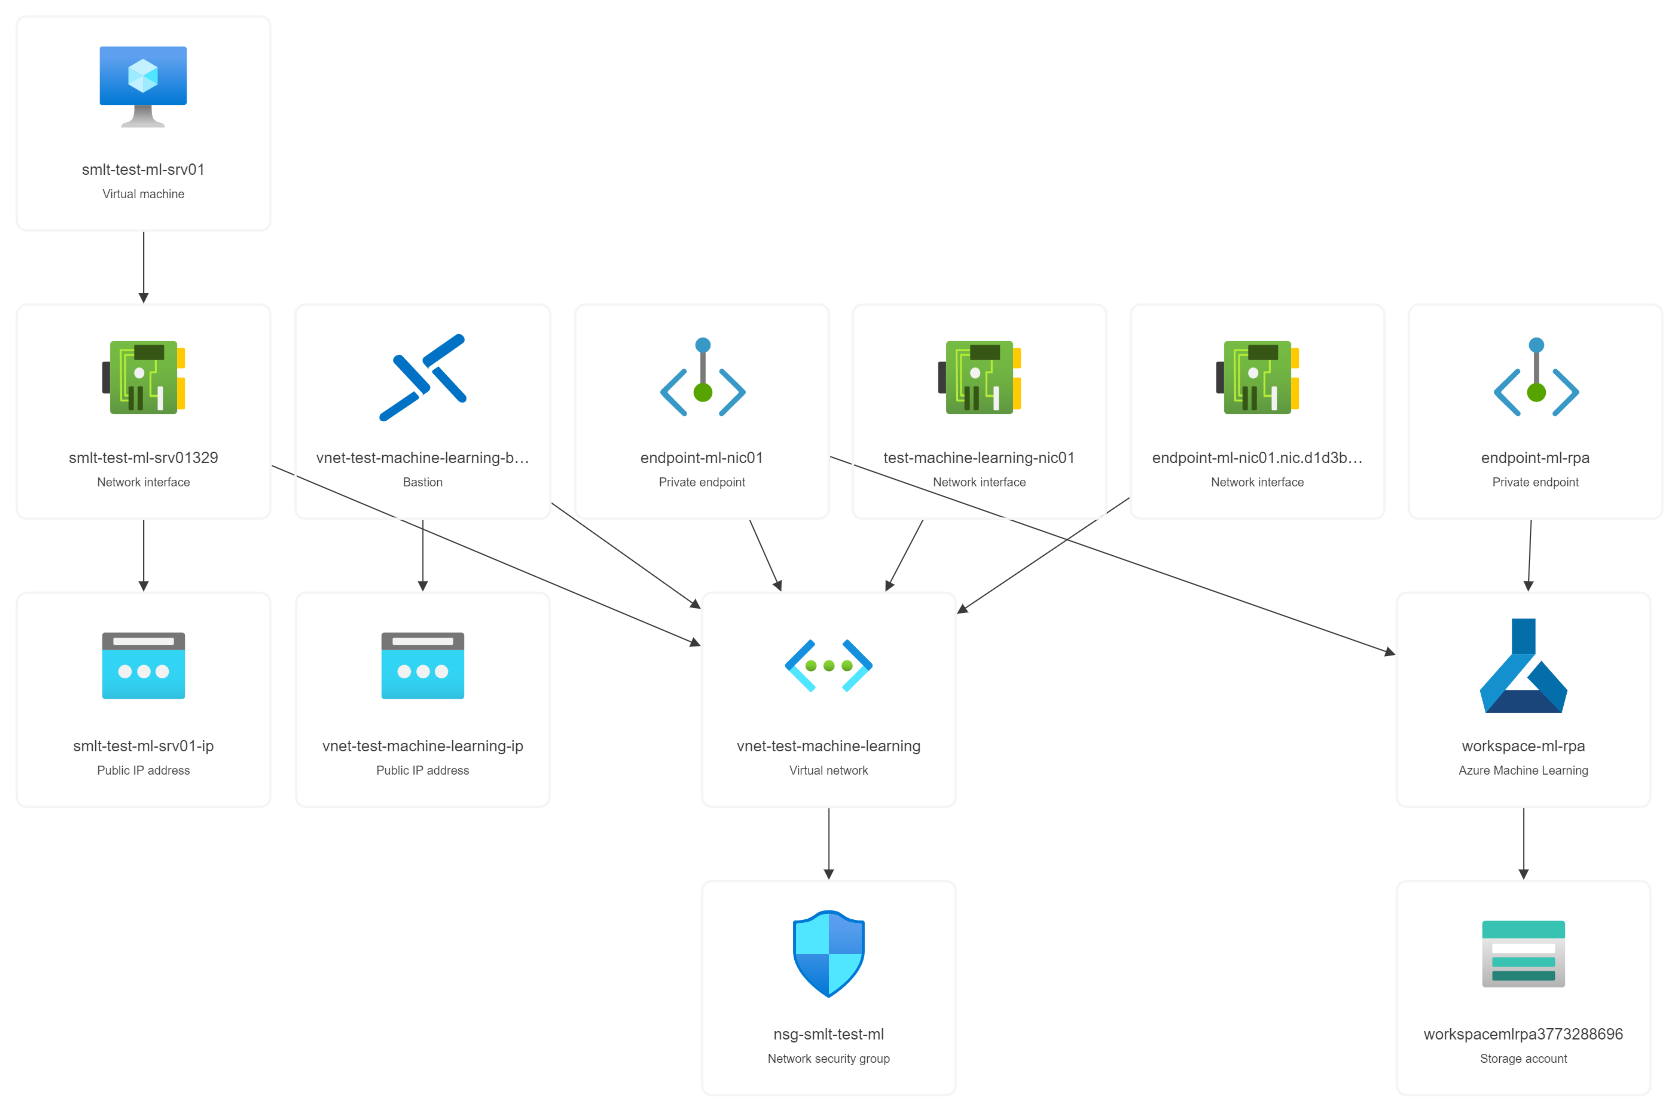
\includegraphics[width=\textwidth]{./appendices/azure-resource-diagram}
    \caption{Azure cloud resources needed and their relations
    \label{fig:azure-diagram}}
\end{figure}

Storage account \textit{worspacemlrpa}
was linked to the Azure Machine Learning workspace.
This storage is the main disk
that stores all the input data used for algorithm training
as well as the result data from said algorithms.
Virtual network \textit{vnet-test-machine-learning}
is the mentioned network
that includes both ML workspace and virtual machine
used to access the ML Studio web UI\@.
Private endpoint \textit{endpoint-ml-nic01}
acted as a final link between ML workspace and virtual network.


%% ............................................................................................................

\subsection{Azure ML Studio}\label{subsec:meth-azure-ml-studio}

The actual machine learning pipeline design and algorithm training
is done with ML Studio portal,
which is a graphic web user interface.
It is a separate tool usable outside usual Azure environment
after configuring the workspace in Azure resources.
Inside ML Studio,
there are two important resources needed to set up
before pipeline designing can start.

First,
the data have to be registered as an usable asset.
Multiple pre-existing data sources are available to choose
from online sources,
and designer can also choose to use
other accessible web file sources.
Besides these,
datasets can be imported from Azure datastore accounts.
Data can be uploaded from local machine through the Studio UI
so it is saved to the chosen datastore.
As datastores are usable with all Azure service resources,
it is possible to use data gathered from any other Azure service
for machine learning training.
In this study,
the data anonymized and preprocessed in local machine
was imported with a separate Azure software to the storage account
and registered as ML dataset from Studio UI.

In addition to the data we used to train the algorithm,
we needed to set up computing instance
in Azure ML studio.
Some predefined resource limitations
affected the computing instance choosing.
After encountering some memory related issues in pipeline training,
we were encouraged to pick memory prioritized instances.
Single computing instance did not work,
but we needed to choose a computing cluster instead
to be able to run ML training pipeline.
After choosing suitable virtual machine properties for compute cluster instances,
a number of nodes is possible to set.
Each of these nodes are a copy of the virtual machine
chosen in the previous step.
If more than one node is chosen,
computing cluster scales to use more nodes
depending on the ML training demands.

For the purposes of this study,
we chose to use maximum two nodes.
The virtual machine properties chosen
were 4 core machine with 28 GB of RAM and 200 GB of disk space.


\clearpage